\فصل{مقدمه}\برچسب{فصل‌مقدمه}\صفحه‌جدید\صفحه‌پاک
\قسمت{ مقدمه ای بر رایانش ابری}
 امروزه با پیشرفت روز افزون فناوری اطلاعات و افزایش برنامه‌های کاربردی، 
 بی‌شک نیاز به محاسبات مسنجم و یکپارچه برای کاربران ضروری می‌باشد.
 همچنین با توجه به نیازهای کاربردی که کاربران دارند، 
 نیاز است که کاربران بتوانند کارهای پیچیده خود را بدون  اینکه 
 نیازی به داشتن سخت افزارها و نرم‌افزارهای گران قیمت داشته باشند، 
 از طریق اینترنت بتوانند انجام دهند. در واقع با این پردازش‌های سخت و سنگین، 
 نیاز به پردازنده‌های متنوع و زیاد دارند تا بتوانند این کارهای پیچیده را با آنها انجام دهند. بنابراین استفاده از تکنولوژی مانند رایانش ابری که با توجه به نیاز کاربران، پردازش‌های محاسباتی آن‌ها آن‌ها را انجام دهد و نتایج را به آن‌ها 
 نمایش دهد، لازم می‌باشد. سیستم‌های رایانش ابری مراکز داده را با طراحی به صورت شبکه‌های مجازی، از نظر سخت‌افزار، پایگاه‌داده، نرم‌افزار و... توانمند کردند، 
 به‌طوری‌که کاربران بتوانند برنامه‌های کاربردی و موردنیاز خود را از هر جایی  با کمترین هزینه دریافت کنند.
  \cite{define,num2}
  
  انجمن ملی استاندارها و تکنولوژی سیستم‌های رایانش ابری را اینگونه تعریف می‌کند: سیستم‌های رایانش ابری مدلی برای فراهم کردن دسترسی آسان بر طبق نیاز کاربران به مجموعه ای از منابع که قابل تغییر از طریق اینترنت هستند، می‌باشد.
  \cite{define}
  \قسمت{ لایه‌ها و سرویس‌های سیستم‌های رایانش ابری}


   سیستم‌های رایانش ابری از مجموعه ای از لایه‌ها تشکیل شده است که برنامه‌های کاربران بر روی این لایه‌ها نصب و اجرا می‌گردد. این لایه‌ها در سه سطح متفاوت به نام‌های زیرساخت تحت یک سرویس
   \پانویس{
\lr{Infrastructure as a Service}   
}
  \lr{  (IaaS)}
    ، پلت‌فرم تحت یک سرویس
    \پانویس{
\lr{Platform as a Service}    
} 
   \lr{ (PaaS)}
     و نرم ‌افزار تحت یک سرویس
     \پانویس{
 \lr{Software as a Service}    
 } 
  \lr{  (SaaS)}
     ارائه می‌شوند. در زیر به معرفی هر سرویس می‌پردازیم:

   \شروع{شمارش}
\فقره سطح اول که با 
\lr{IaaS}
 شناخته می‌شود ، سرویس‌های زیرساخت ابری نام دارد که سیستمی‌ را که عموما به صورت یک بستر مجازی‌سازی شده می‌باشد را به صورت سرویس ارائه می‌دهند. در این سطح، کاربران به جای خرید سخت‌افزار ، نرم‌افزار و تجهیزات شبکه، تمام این امکانات و زیر ساخت‌ها را به صورت یک سرویس مجازی خریداری می‌کنند. درواقع تجهیزات مورد نیاز براساس یک مدل که بر پایه قیمت گذاری براساس استفاده آن‌ها از منابع می‌باشد، ارائه می‌شود.از آنجا که این منبع ممکن است تغییر کند، این چارچوب هم به صورت پویا براساس نیاز به منابع تغییر می‌کند. نمونه ارائه کننده این سرویس‌ها مانند شرکت آمازون می‌باشد.
   
\فقره در سطح بعدی که با 
\lr{PaaS}
  نمایش داده می‌شود، محیطی برای تولید برنامه‌ها و همچنین تست آن‌ها  را فراهم می‌آورد. 
            \begin{figure}
	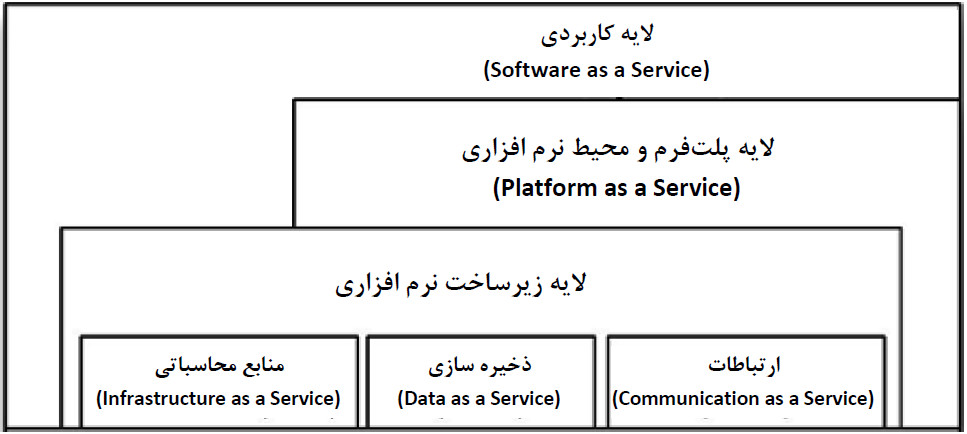
\includegraphics[width=1\textwidth]{files/layers.jpg}
	\caption{لایه‌های سرویس ابری}
\end{figure}
  
\فقره در سطح بعدی که با 
\lr{SaaS}
 نمایش داده می‌شود، در واقع این سطح نرم‌افزاری است که از طریق اینترنت و براساس الگوی قیمت گذاری مشخص شده براساس مصرف کاربر در اختیار آن‌ها قرار داده می‌شود. برای نمونه می‌توانیم به گوگل داک در سایت گوگل اشاره کرد
  \cite{num3,num4}.

   \پایان{شمارش}

\قسمت{ مجازی‌سازی منابع و مفهوم ترکیب در سیستم‌های ابری}
مجازی‌سازی سطح جدیدی از انعطاف پذیری را برای استفاده از منابع ماشین‌های فیزیکی
\پانویس{
	\lr{Physical machine}
}
  \lr{(PM) }
 فراهم می‌کند و امکان یکپارچه سازی منابع فیزیکی   در قالب منابع مجازی  را ایجاد می‌کند. در محیط سیستم‌های رایانش ابری از تکنیک مجازی‌سازی استفاده می‌شود. تکنیک مجازی‌سازی این امکان را فراهم می‌کند که چندین نرم‌افزار که در واقع روی ماشین‌های مجازی
 \پانویس{
\lr{Virtual machine} 
}
 \lr{(VM) }
 قرار داده می‌شوند را همزمان بر روی تنها یک کامپیوتر اجرا کنیم از جمله مهم‌ترین اهداف مجازی‌سازی می‌توانیم به موارد زیر اشاره کنیم.
 \شروع{فقرات}
\فقره{\درشت  بهره‌وری و بهینه سازی در  استفاده از منابع}

با ویژگی مجازی‌سازی، ماشین‌های مجازی می‌توانند یکپارچه شوند و به سیستم‌های بیکار یا در حال استفاده فرستاده شوند. با استفاده از مجازی‌سازی، سیستم‌های موجود می‌توانند یکپارچه شوند. در واقع مجازی‌سازی یک فرصت برای یکپارچه‌سازی و بهینه سازی معماری سیستم‌ها، زیرساخت برنامه‌ها، پایگاه‌های داده، را فراهم می‌آورد که کارایی بالاتر را نتیجه می‌دهد.
 \فقره {\درشت کمتر مصرف کردن برق و در نتیجه کاهش هزینه‌ها 	}
 استفاده از مجازی‌سازی این امکان را فراهم می‌آورد که میزان انرژی مصرفی کاهش یابد و در هزینه‌ها و سرمایه‌های استفاده شده به طور قابل توجهی صرفه جویی به عمل آید.
 \فقره{\درشت صرفه‌جویی شدن در فضا }
  بزرگ بودن و جاگیر بودن سرورهای فیزیکی یک مساله بزرگ در مراکز داده ابری می‌باشد. مجازی‌سازی می‌تواند این مشکل را با یکپارچه‌کردن تعداد زیادی ماشین‌های مجازی بر روی تعداد کمی‌میزبان‌های فیزیکی بر طرف کند.
   \پایان{فقرات}
  
  در سیستم‌های مجازی‌سازی ما از مفاهیمی‌مانند ماشین‌مجازی، ماشین فیزیکی، مهاجرت و ترکیب
  \پانویس{
\lr{Consolidation }  }
     استفاده می‌کنیم. طبق بیانات قبلی،  ماشین‌مجازی مانند یک سیستم واقعی است که بر روی این ماشین می‌توانیم نرم‌افزارها و یا سیستم‌عامل‌های مورد نیاز کاربران را نصب کنیم. بعد از نصب نرم‌افزارها و یا سیستم‌عامل‌های مورد نظر روی این ماشین‌های مجازی، در نهایت این ماشین‌های مجازی بر روی یک ماشین فیزیکی که در واقع یک سرور کامپیوتری با قابلیت‌های بالایی است، اجرا می‌شود. هر ماشین فیزیکی می‌توانید به‌طور همزمان چندین ماشین‌مجازی با نیاز به منابع متفاوت را بر روی خودش اجرا کند. بین ماشین‌های فیزیکی زمانی که یک ماشین فیزیکی بار زیادی روی آن قرار بگیرد و منابع لازم را برای ماشین‌مجازی نداشته باشد، از امکانی به نام مهاجرت در بین ماشین‌های فیزیکی می‌توانیم استفاده کنیم. در واقع از این امکان برای انتقال ماشین‌های مجازی برای اینکه بتوانیم از منابع ماشین‌های فیزیکی به گونه‌ای مناسب استفاده کنیم، استفاده می‌شود. با مهاجرت ماشین‌های مجازی می‌توانیم ماشین‌های مجازی را تا جای ممکن که آن ماشین فیزیکی ظرفیت دارد بر روی آن قرار دهیم و از منابع ماشین فیزیکی حداکثر استفاده را بکنیم و ماشین‌های فیزیکی اضافه را خاموش کنیم، به این عمل ترکیب گفته می‌شود. در واقع این روش تکنیک موثری است که با بالا بردن بهره‌وری از منابع و حداقل کردن تعداد ماشین‌های فیزیکی مصرف انرژی را کاهش می‌دهد. این تکنیک با مهاجرت ماشین‌های مجازی از روی ماشین‌های فیزیکی بیکار به میزبان‌های دیگر و سپس تغییر وضعیت ماشین‌های فیزیکی بیکار به حالت خواب سعی دارد مصرف انرژی را کاهش دهد و از منابع به طور موثری استفاده کند.
\cite{num5,num6,num7}
   
  
  اگرچه ترکیب پویای ماشین‌های مجازی ممکن است کارایی مراکز داده را بهبود بخشد، 
  اما به‌دلیل قرار گرفتن چندین ماشین‌مجازی روی یک ماشین فیزیکی، تضمین‌کردن سرویس‌های مورد نظر به کاربران یکی از چالش‌های بزرگ مربوط به این تکنیک می‌باشد. کیفیت سرویس مربوط به کاربران معمولا با توافق نامه سطح خدمات
  \پانویس{
\lr{Service level agreement}  }
    ارائه می‌شود
\cite{num7}

 ترکیب بهینه ماشین‌های مجازی شامل سه بخش می‌باشد:
\شروع{شمارش}
\فقره شناسایی ماشین‌های فیزیکی سربار شده  
\فقره شناسایی ماشین‌های فیزیکی کم‌بار شده
\فقره انتخاب ماشین‌های مجازی برای مهاجرت از ماشین‌های سربار
 \پایان{شمارش}
 \قسمت{پرسش اصلی}
   در این رساله قصد داریم به این پرسش پاسخ دهیم که به چه نحوی عمل جایابی ماشین‌های مجازی را به میزبان‌های فیزیکی انجام دهیم تا از منابع میزبان‌های فیزیکی به گونه ای مناسب استفاده کنیم تا بتوانیم در بهبود کیفیت سرویس و توان مصرفی موثر واقع شویم.
 \قسمت{تعریف مساله}
 امروزه با چالش‌های متنوعی در زمینه سیستم‌های رایانش ابری مواجه هستیم که یکی از این چالش‌ها چگونگی تخصیص منابع به منظور بهبود کیفیت سرویس و کاهش مصرف انرژی در  مراکز داده ابری می‌باشد. افزایش مصرف انرژی در سیستم‌های رایانش ابری اثرات مخربی از جمله  افزایش گرمای جهانی، آلودگی محیط و ... را در پی خواهد داشت.  برای بیان مسئله خود در این تحقیق ما به دنبال راهکاری هستیم تا از سرریز شدن میزبان‌های فیزیکی جلوگیری کنیم. به این دلیل که سرریز شدن میزبان‌های فیزیکی نقض کیفیت سرویس را به همراه دارد. در این رساله قصد داریم به این مساله بپردازیم که تخصیص ماشین‌های مجازی به میزبان‌های فیزیکی را به چه نحوی انجام دهیم که تا جای ممکن از سریز شدن میزبان‌های فیزیکی با تخصیص مناسب ماشین‌های مجازی روی آن‌ها جلوگیری کنیم.همچنین به منظور مهاجرت ماشین‌های مجازی کنترلی روی آن‌ها به منظور مدیریت موثرتر صورت داده‌ایم.
 \قسمت{اهداف تحقیق به صورت کلی و جزئی}
  هدف ما در این پایان نامه ارائه روشی برای کاهش میزبان‌های فیزیکی سریز شده به منظور جلوگیری از نقض کیفیت خدمات و کاهش توان مصرفی می‌باشد. برای این منظور قصد داریم  با جایابی بهینه ماشین‌های مجازی تا جای ممکن از سریز شدن میزبان‌های فیزیکی جلوگیری کنیم. همچنین قصد داریم با کنترل مهاجرت، در بهبود مصرف انرژی و کیفیت سرویس تاثیر بگذاریم. 
  \قسمت{فرضیه‌های تحقیق}
  \شروع{فقرات}
\فقره  در محیط مورد نظر فرض کردیم ماشین‌های مجازی و میزبان‌های فیزیکی از یک نوع نیستند.یعنی محیط ناهمگن است.
 \فقره درخواست‌ها هیچ وابستگی به هم ندارند و مستقل هستند
 \فقره هر درخواست روی یک ماشین‌مجازی قرار می‌گیرد.
 \پایان{فقرات}
 \قسمت{ابزارهای اندازه‌گیری}
 برای ارزیابی روش پیشنهادی خود آن را با شبیه ساز کلادسیم مورد بررسی و ارزیابی قرار داده ایم .
 \قسمت{جنبه نوآوری و جدید بودن تحقیق در چیست}
   در واقع قصد داریم با قرار دادن مناسب ماشین‌های مجازی به میزبانی که منابع لازم را برای آن ماشین‌مجازی دارد از اضافه باری آن میزبان جلوگیری کنیم. همچنین اگر میزبانی در آینده دچار اضافه باری شد با اعمال سیاستی مناسب برای انتخاب ماشین‌مجازی از آن میزبان بتوانیم در بهبود کیفیت سرویس موثر تر واقع شویم.
   \قسمت{مراحل پایان‌نامه}
   در ادامه تحقیق، در فصل دوم به بررسی روش‌های قبلی بیان شده در زمینه کیفیت سرویس و مصرف انرژی می‌پردازیم. در فصل سوم، روش پیشنهادی به طور کامل شرح داده می‌شود. سپس در فصل چهارم به بررسی و ارزیابی روش پیشنهادی و کار مورد مقایسه می‌پردازیم. در نهایت، در فصل پنجم به جمع‌­بندی پایان نامه و کارهای آینده می‌پردازیم.
   




